\subsection{x86}

\subsubsection{\NonOptimizing MSVC}

Имеем в итоге (MSVC 2010):

\lstinputlisting[caption=MSVC 2010]{patterns/14_bitfields/2_set_reset/set_reset_msvc.asm}

\myindex{x86!\Instructions!OR}
Инструкция \OR здесь устанавливает в переменной ещё один бит, игнорируя остальные.

\myindex{x86!\Instructions!AND}
А \AND сбрасывает некий бит. Можно также сказать, что \AND здесь копирует все биты, кроме одного. 
Действительно, во втором операнде \AND выставлены в единицу те биты, которые нужно сохранить, 
кроме одного, копировать который мы не хотим (и который 0 в битовой маске).
Так проще понять и запомнить.

\clearpage
\myparagraph{\olly}

Попробуем этот пример в \olly.
Сначала, посмотрим на двоичное представление используемых нами констант:

\TT{0x200} (0000000000000000000{\color{red}1}000000000) (т.е. 10-й бит (считая с первого)).

Инвертированное \TT{0x200} это \TT{0xFFFFFDFF} (1111111111111111111{\color{red}0}111111111).

\TT{0x4000} (00000000000000{\color{red}1}00000000000000) (т.е. 15-й бит).

Входное значение это: \TT{0x12340678} (10010001101000000011001111000).
Видим, как оно загрузилось:

\begin{figure}[H]
\centering
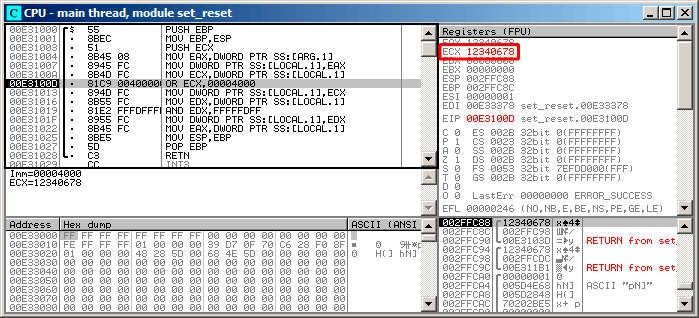
\includegraphics[scale=\FigScale]{patterns/14_bitfields/2_set_reset/olly1.png}
\caption{\olly: значение загружено в \ECX}
\label{fig:set_reset_olly1}
\end{figure}

\clearpage
\OR исполнилась:

\begin{figure}[H]
\centering
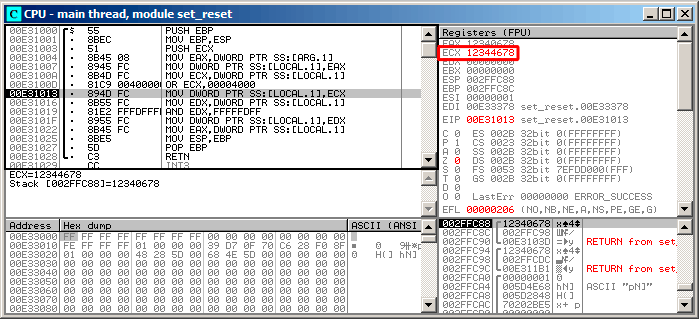
\includegraphics[scale=\FigScale]{patterns/14_bitfields/2_set_reset/olly2.png}
\caption{\olly: \OR сработал}
\label{fig:set_reset_olly2}
\end{figure}

15-й бит выставлен: \TT{0x1234{\color{red}4}678} 
(10010001101000{\color{red}1}00011001111000).

\clearpage
Значение перезагружается снова (потому что использовался режим компилятора без оптимизации): 

\begin{figure}[H]
\centering
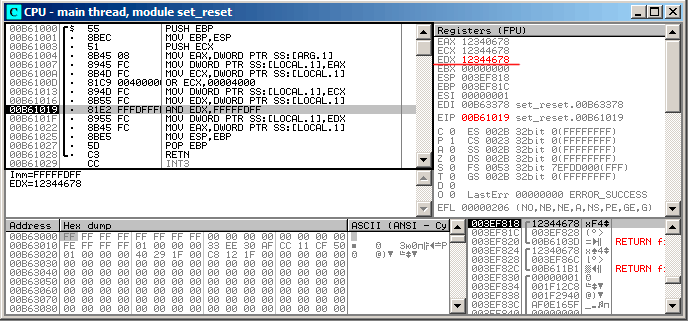
\includegraphics[scale=\FigScale]{patterns/14_bitfields/2_set_reset/olly3.png}
\caption{\olly: значение перезагрузилось в \EDX}
\label{fig:set_reset_olly3}
\end{figure}

\clearpage
\AND исполнилась:

\begin{figure}[H]
\centering
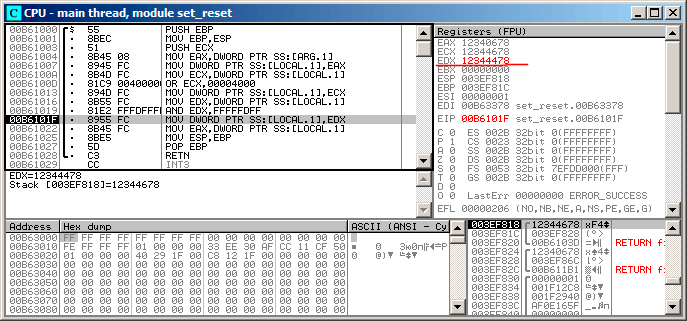
\includegraphics[scale=\FigScale]{patterns/14_bitfields/2_set_reset/olly4.png}
\caption{\olly: \AND сработал}
\label{fig:set_reset_olly4}
\end{figure}

10-й бит очищен (или, иным языком, оставлены все биты кроме 10-го) и итоговое значение это \\
\TT{0x12344{\color{red}4}78} (1001000110100010001{\color{red}0}001111000).

\subsubsection{\Optimizing MSVC}

Если скомпилировать в MSVC с оптимизацией (\Ox), то код еще короче:

\lstinputlisting[caption=\Optimizing MSVC]{patterns/14_bitfields/2_set_reset/set_reset_msvc_Ox.asm}

\subsubsection{\NonOptimizing GCC}

Попробуем GCC 4.4.1 без оптимизации:

\lstinputlisting[caption=\NonOptimizing GCC]{patterns/14_bitfields/2_set_reset/set_reset_gcc.asm}

Также избыточный код, хотя короче, чем у MSVC без оптимизации.

Попробуем теперь GCC с оптимизацией \Othree:

\subsubsection{\Optimizing GCC}

\lstinputlisting[caption=\Optimizing GCC]{patterns/14_bitfields/2_set_reset/set_reset_gcc_O3.asm}

Уже короче. Важно отметить, что через регистр \AH компилятор работает с частью регистра \EAX. 
Это его часть от 8-го до 15-го бита включительно.

\RegTableOne{RAX}{EAX}{AX}{AH}{AL}

\myindex{Intel!8086}
\myindex{Intel!80386}
N.B. В 16-битном процессоре 8086 аккумулятор имел название \AX 
и состоял из двух 8-битных половин~--- \AL (младшая часть) и \AH (старшая). 
В 80386 регистры были расширены до 32-бит, 
аккумулятор стал называться \EAX, но в целях совместимости, к его \IT{более старым} частям всё ещё можно 
обращаться как к \AX/\AH/\AL.

Из-за того, что все x86 процессоры~--- наследники 16-битного 8086, эти \IT{старые} 16-битные опкоды короче 
нежели более новые 32-битные. 
Поэтому инструкция \INS{or ah, 40h} занимает только 3 байта. 
Было бы логичнее сгенерировать здесь \INS{or eax, 04000h}, но это уже 5 байт, или даже 6 
(если регистр в первом операнде не \EAX).

\subsubsection{\Optimizing GCC и regparm}

Если мы скомпилируем этот же пример не только с включенной оптимизацией \Othree, 
но ещё и с опцией \TT{regparm=3}, о которой я писал немного выше, то получится ещё короче:

\lstinputlisting[caption=\Optimizing GCC]{patterns/14_bitfields/2_set_reset/set_reset_gcc_O3_regparm3.asm}

\myindex{Inline code}
Действительно~--- первый аргумент уже загружен в \EAX, и прямо здесь можно начинать с ним работать. 
Интересно, что и пролог функции (\INS{push ebp / mov ebp,esp}) и эпилог (\INS{pop ebp}) 
функции можно смело выкинуть за ненадобностью, 
но возможно GCC ещё не так хорош для подобных оптимизаций по размеру кода. 
Впрочем, в реальной жизни подобные короткие функции лучше всего автоматически делать в виде 
\IT{inline-функций} (\myref{inline_code}).

